\documentclass{article}


\usepackage{arxiv}

\usepackage[utf8]{inputenc} % allow utf-8 input
\usepackage[T1]{fontenc}    % use 8-bit T1 fonts
\usepackage{hyperref}       % hyperlinks
\usepackage{url}            % simple URL typesetting
\usepackage{booktabs}       % professional-quality tables
\usepackage{amsfonts}       % blackboard math symbols
\usepackage{nicefrac}       % compact symbols for 1/2, etc.
\usepackage{microtype}      % microtypography
\usepackage{lipsum}
\usepackage{graphicx}
\usepackage{longtable}


\graphicspath{ {./images/} }


\title{AI-based SuPport algorIthm foR rEal-time pollen monitoring IoT system (ASPIRE)}


\author{
 Slobodan Jelić \\
  Faculty of Civil Engeneering\\
  University of Belgrade\\
  Bulevar Kralja Aleksandra 73,
  11000, Belgrade \\
  Serbia\\
  \texttt{sjelic@grf.bg.ac.rs} \\
  %% examples of more authors
   \And
 Predrag Matavulj \\
  Biosense Institue\\
  Dr Zorana Đinđića 1\\
  21000 Novi Sad\\
  Serbia\\
  \texttt{matavulj.predrag@biosense.rs} \\
  \And
 Domagoj Ševerdija \\
  J. J. Strossmayer university of Osijek\\
  Department of Mathematics\\
  Trg Ljudevita Gaja 6 \\
  31000 Osijek\\
  Croatia\\
  \texttt{dseverdi@mathos.hr}
}
\begin{document}
\maketitle



% keywords can be removed
%\keywords{First keyword \and Second keyword \and More}

\section{Data description}

We start with two datasets: a real-time dataset acquired from an instrument in real time, and a calibration dataset created under laboratory conditions. Both data sets were generated using the Rapid-E instrument from Plair SA \cite{kiselev_flash-lamp_2013}, which is based on the concept of two-phase particle analysis: UV laser for the scattering signal and deep UV for the laser-induced fluorescence. It is known that scattering correlates with particle morphology (size and shape), while fluorescence for spectrum and lifetime provides information about particle chemical properties. This provides an efficient filter for pollen particles, as pollen particles are expected to have a fluorescence intensity greater than $1500$ units.

\section{Model Architecture}

The original deep neural network model is based on the architecture presented in \cite{sauliene_automatic_2019}. The scattered signal is processed with a two-dimensional convolutional block, followed by batch normalization and a fully connected layer at the end. The authors introduced two-dimensional convolutional layers because the scattering signal can be interpreted as a two-dimensional image. Spectrum and lifetime signals, on the other hand, are processed with multiple convolutional blocks followed by a fully connected layer. The extracted features at the end of the convolution blocks are merged and passed to a fully connected layer, followed by a sigmoid function that converts the outputs into probabilities (Figure \ref{fig::arch}).

\begin{figure}
  \centering
  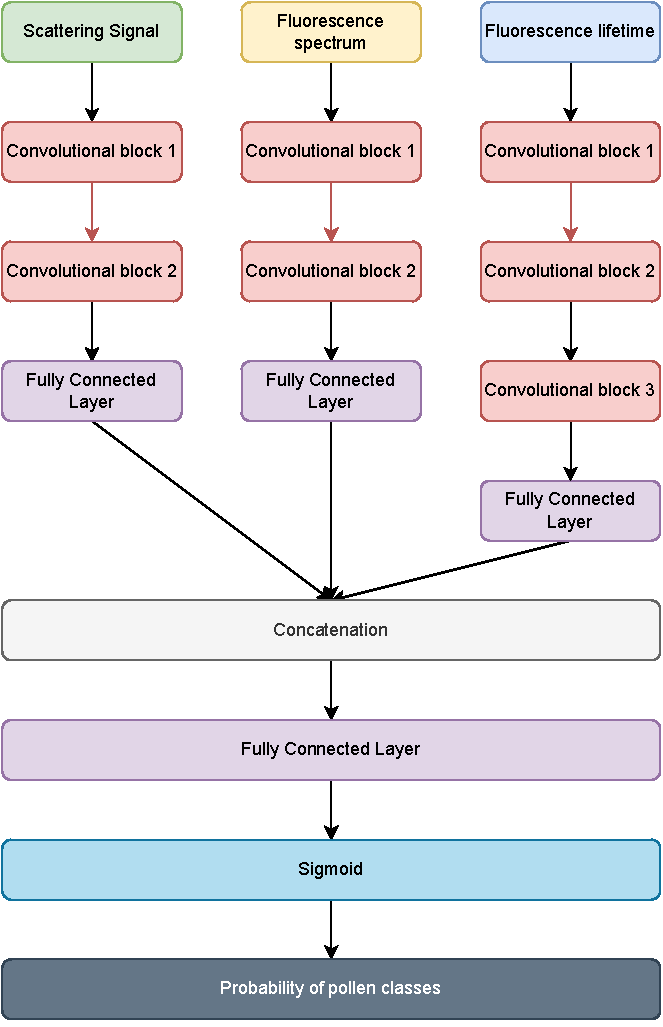
\includegraphics[width=0.7\textwidth]{arch.pdf}
  \caption{Model architecture in \cite{sauliene_automatic_2019}}\label{fig::arch}
\end{figure}

More specifically, the two-dimensional convolutional block for input scattering signals consists of two-dimensional convolutional layers, replication padding layers, ReLU activation functions, batch normalization layers, max-pooling, and dropout layers (Figure \ref{fig::conv}).

\begin{figure}
  \centering
  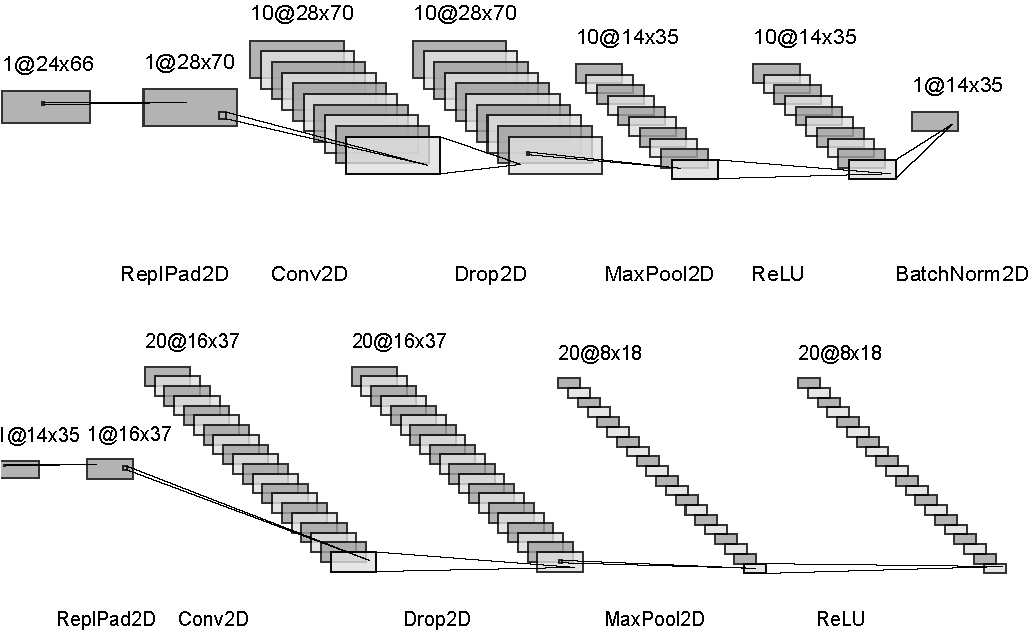
\includegraphics[width=0.9\textwidth]{convblock.pdf}
  \caption{Convolutional block for scattering signal}\label{fig::conv}
\end{figure}

In the preprocessing phase, we also introduce particle size, which can be directly derived from the scattering signal. Particle size correlates strongly with the class of pollen grains in the air, but is not sufficient for accurate classification because different pollen types have the same size.



\section{Objective loss}

The weighted cross entropy function is used for the training objectives of the model. The weights are inversely proportional to the pollen class frequencies (target variable) to account for the imbalance of class frequencies in the data set.

\section{Training process}

The stochastic gradient descent method is used to train the model with a weight-decay parameter to control overfitting of the model. Also, the training data set is split into a training data set and a validation data set, where the validation data set is used to control the overfitting during the training process. The size of the batches is determined by the available computational resources. The batches are determined by a stratified partitioning strategy with respect to the frequency of pollen classes in the training dataset. In other words, the batch is a stratified subsample of the entire training dataset with respect to the frequency of pollen classes in the target variable.

The standard backpropagation algorithm is used to compute the direction of gradient descent, while the learning rate is set as a hyperparameter.
At each epoch, we determine if the current model in the validation set has better accuracy than the current best model. If so, we save this model as the best one found and continue training until the maximum number of epochs is reached.

\section{Hyperparameter tuning and cross-validation}

To avoid overfitting, we perform nested $k$-fold cross-validation with a stratified split strategy. In inner cross-validation, the training dataset is split into a training dataset and a validation dataset. The validation dataset is used to measure the performance of the model for a given grid search point (i.e., a combination of hyperparameters). Finally, we select the trained model with the combination of hyperparameters that has the best performance on the validation dataset. This model is evaluated with a test set from the outer cross-validation.
When reporting model performance, we report the mean and standard deviation of model accuracy over $k$ folds in the outer cross-validation.

Finally, the model is re-trained with the best combination of hyperparameters on the entire dataset.



\section{Platform}
For training, we use a high-performance server with multiple GPUs and installation of Python, Pytorch, and Tensorboard packages.

\section{Evaluation}

In the first phase of the project, we consider a multi-class model from the literature with poor performance of about $30\%$ classification accuracy. Since the training process is time consuming, we installed TensorBoard locally to track the learning process and evaluation metrics on different datasets 

\section{Plans for improvement}
To improve this accuracy, we will apply the transfer learning paradigm of this model trained on the calibration set to the domain of unlabeled data available during the Rapid-E deployment during the season in the city of Osijek. This dataset consists of unlabeled measurements for each particle, and we do not know whether that particle is pollen or not. However, we have access to information on the number of pollen particles in a given time period (usually 1 hour) measured by the Hirst instrument. These data can be used to improve the classification accuracy of the model by introducing a new objective loss that penalizes higher deviations from the reliable number of pollen grains.

\section{Code repository}

The code produced in the first phase of the project is available in the Github repository: \url{https://github.com/sjelic/aspire}.


\bibliographystyle{plain}
\bibliography{references}
\end{document}
